\documentclass[11pt]{article}
\usepackage{StyleSheet}
\usepackage{tikz}
\usetikzlibrary{external}
\tikzexternalize[prefix=Graphs/tikz/]

\begin{document}

\begin{titlepage}
    \centering
    \Huge \textbf{\TITLENAME}
    
    \vspace{1cm}
    
    \Large \NAMES
    
    \vspace{0.5cm}
    
    \large \SCHOOLNAME
    
    \vfill
    
    \today
    
\end{titlepage}

% ---------- %

\renewcommand{\contentsname}{Contents}
\tableofcontents
\newpage

% ---- Preamble End ---- %

\section{Introduction}
Our project is about a vehicle (also referred to as a system) that has the ability to complete an obstacle course test as well as a pickup and placement test in a multitude of ways. On the obstacle course that is outline by white lines on the side and green tape on the front and back end, our vehicle will be able to stay within the white lines and detect the walls within the course, maneuver around them and stop on the green line at the end of the course. For the pickup and placement course our vehicle will be able to detect an I-Beam, pick up a colored box and based on its color and size, drop the box off on the other end of the course and return to starting side of the court. Completing these test requires communication skills, an array of engineering skills such as computer and electrical skills, writing skills, and decision making skills. The intention of the project is to strengthen all of the required skills needed to solve a complex problem that meets the demand being asked. 

The purpose of the report is to detail the process of creating a system that will meet all requirements. The report was also a great way to get the team’s ideas flushed out and catch mistakes within our project that we could then correct. Section 2, the Project Management Plan keeps is a timeline of the system’s progress by giving weekly updates that include the team member(s) who is responsible for the task and the duration of the task. Another key part of the report is Section 3. In this part of the report, the system requirements for certain objectives such as the obstacle avoidance and pickup and placement of the vehicle are established. Other major sections of our report is section 5 and section 7. Section 5 outlines the conceptual designs that the team came up and section 7 details the design of the system which includes algorithms and other electrical and computer engineering tools that were used in the project. Lastly, section 8 goes into depth about the System Test and Verifications also known as T.E.M.P.S.
In this section, an explanation of how each system requirement is tested is provided. 
\documentclass{article}
\usepackage{StyleSheet}
\begin{document}

\section{Project Management Plan}

\end{document}
\documentclass{report}
\usepackage{StyleSheet}
\begin{document}

\chapter{System Requirements}\label{ch:system-requirements}

The overall objective of the system our team has built involves numerous requirements that helped us achieve our objectives. One of the main goals will be for the vehicle to complete the obstacle course in a timely fashion that avoids walls and does not pass specific colored tape. The other main goal will be for the obstacle to pick up a specific colored box, and then follow a particular line of color of the box to a drop-off site, where the vehicle will place the box back down.

\section{Box Pick-up and Placement System}

\subsection{Recognition of the I-Beam}
The vehicle shall find the I-Beam on the course.

\subsection{Orientation of the I-Beam}
The vehicle shall orientate/center itself with the I-Beam

\subsection{Apprehend the Box}
The vehicle shall apprehend the box with the gripper.

\subsection{Identify the Color of the Box}
The vehicle shall identify the color of the box.

\subsection{Identify the Size of the Box}
The vehicle shall identify the size of the box. 

\subsection{Realign with the Line Following Course}
The vehicle shall move itself back onto the line following the course after it has apprehended the box.

\subsection{Follow the Line of the Color of the Box and Return.} 
The vehicle shall follow the colored line of the box’s color it has apprehended.

\subsection{Placement of the Box}
The vehicle shall place the box on the appropriate I-Beam based on the color and size of the box.

\section{Drive Train \& Steering System}

\subsection{Move Forward}
The vehicle shall move forward in a straight line.

\subsection{Move Backward}
The vehicle shall move backward in a straight line.

\subsection{Move Right}
The vehicle shall move right in a straight line.

\subsection{Move Left}
The vehicle shall move left in a straight line.

\subsection{Rotational Movement}
The vehicle shall rotate to the right or left.

\section{Sensor Requirement: IR Sensor Array}

\subsection{Width of the IR Sensors}
The width of the \gls{IR} Array shall be bigger than the width of the tape.

\subsection{The number of sensors is greater than 6}
The amount of sensors on the \gls{IR} Array is greater than 6.

\subsection{It Must Detect and Distinguish the Tape and Tarp}
The \gls{IR} Array must be able to distinguish between the colored tape and the black tarp.

\subsection{It Must be able to Calculate Error}
The \gls{IR} Array must be able to calculate the error to recognize which way the vehicle is deviating.

\subsection{Deviation Adjustment}
The vehicle shall properly correct the vehicle if it deviates from the red, blue, or green line.

\section{Task-2 Completion Times (Obstacle Course)}

\subsection{Detection of Walls }
The vehicle shall detect the walls of the obstacle course via ultrasonic sensors
\subsection{Avoidance of Walls}
The vehicle shall move forward and avoid the walls of the obstacle course by the system not touching any part of the wall. 

\subsection{Detection of Side Boundaries of Obstacle Course via Color Sensors}
The vehicle shall have color sensors that will identify when the system is at the side boundaries of the course. For this specific test, the side boundary is outlined by white tape.

\subsection{Stay within the Obstacle Course Until Course is Complete}
The vehicle’s center of mass shall not deviate outside the side boundary and stay within the obstacle course until completion. 

\subsection{Detection of the Finish Line of Obstacle Course via Color Sensors}
The vehicle shall have color sensors that will identify when the system is at the side boundaries of the course. For this specific test, the side boundary is outlined by white tape.

\subsection{System Stops at the End of the Course}
The vehicle shall detect the green line and fully cross the line, and then stop. 


\end{document}
\documentclass[11pt]{report}
\usepackage{StyleSheets/main}
\begin{document}

\chapter{CONOPs (Concept of Operations)}\label{ch:conops}
The purpose of this section is to provide the user of the robot with a clear and concise description of how this system is operated. The \gls{CONOP}s provides a clear summary of how the vehicle will reach its objective. 
\section{System Summary}
\begin{itemize}
    \item This system is a vehicle with the ability to move right, left, forwards, backwards, and rotate. This vehicle is powered by a battery and controlled using a microcontroller.
    \item The vehicle has a gripper with an arm that allows it to reach for \& pick up objects. 
    \item This vehicle can detect colors, obstacles, and lines.
\end{itemize}
\section{Initialization of the System}
\begin{itemize}
    \item Firstly, the \gls{ABHS} will be placed down on a flat surface, preferably the floor as it takes away the risk of the vehicle falling from a dangerous height.
    \item If the use of the \gls{ABHS} is to fulfill one of its requirements (Obstacle Avoidance, Pickup and Place System with Line Following), then the \gls{ABHS} should be placed in its starting position.
    \item All the connections should be secure and in accordance with the pin map provided with the vehicle.
    \item If a new version of the code is uploaded, verify that the \texttt{while (!Serial)} portion of the \cref{lst:main-h} has been commented out.
    \item Ensure that any external connections the the Teensy 4.1 are terminated to eliminate the possibility of over-powering the Teensy 4.1.
    \item The battery should at this point be connected and switched on, with the green lights appearing when the battery is on. The additional blue \gls{LED} will also light up when the battery is turned on.
\end{itemize}

\section{Standard Operating Modes}
\begin{itemize}
\item This system has 2 normal operating modes:
    \begin{itemize}
        \item This system was designed to perform obstacle avoidance. In the event of a wall being placed in front of the system, the vehicle would find a way around the wall as long as white boundary lines outline the obstacle course.
        \item This system was designed to pick up a box and recognize its color. It will then use this color to transport the box over a line of the same color, and place it in the platform dependant on the size of the box/package. It will then return to its starting position.
\end{itemize}
\end{itemize}
\section {External Environment for use of the System}
\begin{itemize}
    \item This system should typically be used in a room temperature, dry environment. This is due to the open wire nature of the \gls{ABHS}, and its use-case of clean-room operation.
\end{itemize}
\section{Standard Maintenance}
\begin{itemize}
    \item The battery for the \gls{ABHS} should always be charged in order for this system to work.
    \item All wires should be maintained in the correct pin ports. If a wire is in the incorrect port, follow the provided pinout \cref{fig:Pinoutmap}.
    \item The vehicle should be kept in dry, stable conditions, and out of direct sunlight as to avoid potential damage to parts.
\end{itemize}
\section{Failure Modes due to Internal Problems}
\begin{itemize}
    \item In the event of the user at any point seeing or smelling smoke coming from the vehicle, shut the battery off as soon as possible. 
    \item In the case of these events, troubleshoot the system to decipher what the problem point was. Start by seeing if any parts of the system are hot, specifically motors, the Teensy 4.1 microcontroller, and the buck converter. If any signs of overheating occur, immediately disconnect the part for further inspection.
    \item Test the possibly damaged component to see if it functions correctly, if not, replace the damaged component.
\end{itemize}
\section{Reaction to External Failure Modes}
\begin{itemize}
    \item If on the obstacle course the vehicle drives into one of the walls, it should find its own way around it. 
    \item If the vehicle exits the testing course, (ie. over the white line), immediately switch the battery off to avoid the vehicle running too far off course \& potentially crashing, damaging the vehicle.
    \item If during the box pickup test the vehicle drops the box, reset the course and try to run the system again. If this fails again, check to ensure that the gear teeth of the gripper are properly connected.
    \item If the vehicle fails to follow the line and veers off the path, turn off the battery and reset the course. 
\end{itemize}
\section{Shutdown of the System}
\begin{itemize}
    \item Make sure the vehicle has fully run the course of its current objective. Turn the battery off and ensure that the system is fully off. If the vehicle is acting erroneously, it can be manually shut off during it's operation, as it is minimally hazardous to operators.
\end{itemize}


\end{document}

\section{Conceptual Design}
\section{System Risk Management}
\section{Detailed Design}
\section{System Test and Verification}
\section{System Analysis and System Performance Metrics}
\section{Summary}
\section{Documentation and Acknowledgments}
\newpage
\section{References}

\newpage
\section{Appendix}

\subsection{Calibration Data}

\subsubsection{Color Sensor Calibration Points}
\documentclass{article}
\usepackage{GraphDefinitions}

\begin{document}

\foreach \sensor in {middleColor, rightColor, leftColor, gripperColor} {
    \ifthenelse{\equal{\sensor}{middleColor}}{ % Middle color shadow opacity
        \def\opacity{0.010}
    }{
        \def\opacity{0.055} % Non middle color shadow opacity
    }
    \def\ballsize{3pt} % Change the size of the balls
                
    \begin{figure}[H]
        \centering
        \begin{tikzpicture}
            \begin{axis}[
                xlabel={Red Frequency},
                ylabel={Green Frequency},
                zlabel={Blue Frequency},
                xlabel style={sloped like x axis}, % Make x label follow the x axis
                ylabel style={sloped like y axis}, % Make y label follow the y axis
                zlabel style={sloped}, % Make z label follow the z axis or make it vertical
                legend pos=north west,
                grid=both,
                grid style={line width=.1pt, draw=gray!10},
                major grid style={line width=.2pt,draw=gray!50},
                minor tick num=5,
                width=0.8\textwidth,
                height=0.65\textwidth,
                view={45}{45}, % Adjust the view angle for better visualization
            ]
            \IfFileExists{code/output_data/color_sensor_calibration/\sensor.csv}{
                % Determine opacity based on sensor

                \addplot3[
                    only marks,
                    scatter,
                    scatter/classes={
                        RED={mark=ball,ball color= red, draw opacity=0, mark size = \ballsize},
                        BLUE={mark=ball,ball color= blue, draw opacity=0, mark size = \ballsize},
                        GREEN={mark=ball,ball color= green, draw opacity=0, mark size = \ballsize},
                        WHITE={mark=ball,ball color= white, draw opacity=0, mark size = \ballsize},
                        BLACK={mark=ball,ball color= black, draw opacity=0, mark size = \ballsize},
                        YELLOW={mark=ball,ball color= yellow, draw opacity=0, mark size = \ballsize}
                    },
                    scatter src=explicit symbolic,
                ] table[
                    x=Red_Freq,
                    y=Green_Freq,
                    z=Blue_Freq,
                    meta = Color,
                    col sep=comma,
                ] {code/output_data/color_sensor_calibration/\sensor.csv};

                % Wall histogram on the left
                \addplot3[
                    only marks,
                    scatter,
                    scatter/classes={
                        RED={mark=*,fill=red, fill opacity=\opacity, draw opacity=0},
                        BLUE={mark=*,fill=blue, fill opacity=\opacity, draw opacity=0},
                        GREEN={mark=*,fill=green, fill opacity=\opacity, draw opacity=0},
                        WHITE={mark=*,fill=gray, fill opacity=\opacity, draw opacity=0},
                        BLACK={mark=*,fill=black, fill opacity=\opacity, draw opacity=0},
                        YELLOW={mark=*,fill=yellow, fill opacity=\opacity, draw opacity=0}
                    },
                    scatter src=explicit symbolic,
                ] table[
                    x expr = 0,  % This sets the x-coordinate to 0
                    y = Green_Freq,  % This sets the y-coordinate to 0
                    z= Blue_Freq,
                    meta = Color,
                    col sep=comma,
                ] {code/output_data/color_sensor_calibration/\sensor.csv};

                % Wall histogram on the right
                \addplot3[
                    only marks,
                    scatter,
                    scatter/classes={
                        RED={mark=*,fill=red, fill opacity=\opacity, draw opacity=0},
                        BLUE={mark=*,fill=blue, fill opacity=\opacity, draw opacity=0},
                        GREEN={mark=*,fill=green, fill opacity=\opacity, draw opacity=0},
                        WHITE={mark=*,fill=gray, fill opacity=\opacity, draw opacity=0},
                        BLACK={mark=*,fill=black, fill opacity=\opacity, draw opacity=0},
                        YELLOW={mark=*,fill=yellow, fill opacity=\opacity, draw opacity=0}
                    },
                    scatter src=explicit symbolic,
                ] table[
                    x = Red_Freq,  % This sets the x-coordinate to 0
                    y expr = 750,  % This sets the y-coordinate to the back wall
                    z= Blue_Freq,
                    meta = Color,
                    col sep=comma,
                ] {code/output_data/color_sensor_calibration/\sensor.csv};

                % Floor histogram
                \addplot3[
                    only marks,
                    scatter,
                    scatter/classes={
                        RED={mark=*,fill=red, fill opacity=\opacity, draw opacity=0},
                        BLUE={mark=*,fill=blue, fill opacity=\opacity, draw opacity=0},
                        GREEN={mark=*,fill=green, fill opacity=\opacity, draw opacity=0},
                        WHITE={mark=*,fill=gray, fill opacity=\opacity, draw opacity=0},
                        BLACK={mark=*,fill=black, fill opacity=\opacity, draw opacity=0},
                        YELLOW={mark=*,fill=yellow, fill opacity=\opacity, draw opacity=0}
                    },
                    scatter src=explicit symbolic,
                ] table[
                    x = Red_Freq,
                    y = Green_Freq,
                    z expr = 0,
                    meta = Color,
                    col sep=comma,
                ] {code/output_data/color_sensor_calibration/\sensor.csv};

                
            }{}
            \end{axis}
        \end{tikzpicture}
        \caption{\sensor \ Sensor Calibration Data in Euclidean Space.}
        \label{fig:\sensor_calibration_data}
    \end{figure}
}

\end{document}

\subsubsection{IR Array Calibration Points}
\documentclass{article}
\usepackage{GraphDefinitions}

\begin{document}

\begin{figure}[H]
\centering
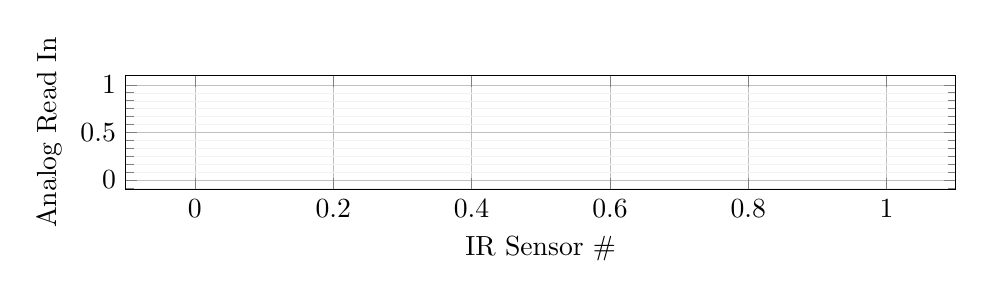
\begin{tikzpicture}
\begin{axis}[
    width=1\textwidth, % Adjust the width as needed
    height=0.25\textwidth, % Adjust the height as needed
    xlabel={IR Sensor \#},
    ylabel={Analog Read In},
    xtick={1, 2, 3, 4, 5, 6, 7}, % Set specific x-axis labels
    legend pos=north west,
    grid=both,
    grid style={line width=.1pt, draw=gray!10},
    major grid style={line width=.2pt,draw=gray!50},
    minor y tick num=5, % This adds the minor grid lines on the y-axis
    minor x tick num=0, % This removes the minor grid lines on the x-axis
    ]
    \IRTrace{green}{Green}{green}
    \IRTrace{blue}{Blue}{blue}
    \IRTrace{red}{Red}{red}
    \IRTrace{yellow}{Yellow}{black}
    \IRTrace{black}{Off}{black}
\end{axis}
\end{tikzpicture}
\caption{IR Calibration Data Based on Tape Color.}
\label{ir-calibration-data}
\end{figure}

\end{document}


\subsubsection{Motor Calibration Points}
\documentclass[12pt]{report}
\usepackage{GraphDefinitions}

\begin{document}

\begin{figure}[H]
\centering
\begin{tikzpicture}
    \begin{axis}[
        title = {Speed Percent ($\% \cdot 100$) vs Speed (cm/s)},
        width=1\textwidth, % Make the plot as wide as the subfigure
        height=0.45\textwidth, % Adjust the height for a wide format
        xlabel={Speed (cm/s)},
        ylabel={Speed Percent ($\% \cdot 100$)},
        legend pos=north west,
        ymin = -10,
        grid=both,
        grid style={line width=.1pt, draw=gray!10},
        major grid style={line width=.2pt,draw=gray!50},
        ]
        \MotorTrace{left}{speed_percent}{Left Speed Percent}{red}{solid}        
        \MotorTrace{right}{speed_percent}{Right Speed Percent}{green}{solid}
        \MotorTrace{top}{speed_percent}{Top Speed Percent}{blue}{solid}
        \MotorTrace{bottom}{speed_percent}{Bottom Speed Percent}{black}{solid}
    \end{axis}
\end{tikzpicture}
\label{speed-calibration-data}
\caption{Motor Calibration Data Regarding Speed Percent}
\end{figure}

\vspace{0.5cm} % Space between the subfigures

\begin{figure}[H]
\centering
\begin{tikzpicture}
    \begin{axis}[
        title = {PWM Percent ($\% \cdot 100$) vs Speed (cm/s)},
        width=\textwidth, % Make the plot as wide as the subfigure
        height=0.45\textwidth, % Adjust the height for a wide format
        xlabel={Speed (cm/s)},
        ylabel={PWM Percent ($\% \cdot 100$)},
        ymin = -10,
        legend pos=north west,
        grid=both,
        grid style={line width=.1pt, draw=gray!10},
        major grid style={line width=.2pt,draw=gray!50},
        ]
        \MotorTrace{left}{pwm_percent}{Left PWM Percent}{red}{solid}        
        \MotorTrace{right}{pwm_percent}{Right PWM Percent}{green}{solid}
        \MotorTrace{top}{pwm_percent}{Top PWM Percent}{blue}{solid}
        \MotorTrace{bottom}{pwm_percent}{Bottom PWM Percent}{black}{solid}
    \end{axis}
\end{tikzpicture}
\label{pwm-calibration-data}
\caption{Motor Calibration Data Regarding PWM Percent}
\end{figure}

\end{document}


\subsection{Color Sensor Euclidean Distance Visualization}
\documentclass[12pt]{report}
\usepackage{GraphDefinitions}

\begin{document}

\def\grayopacity{0.055}
\def\ballsize{3pt} % Change the size of the balls
\def\seencolor{orange}
\def\seenx{543}
\def\seeny{340}
\def\seenz{500}
\def\calix{574}
\def\caliy{271}
\def\caliz{435}
\def\calicolor{blue}
\def\maxy{750}
\def\maxx{825}
\def\shadowopacity{0.4}
            
\begin{figure}[H]
    \centering
    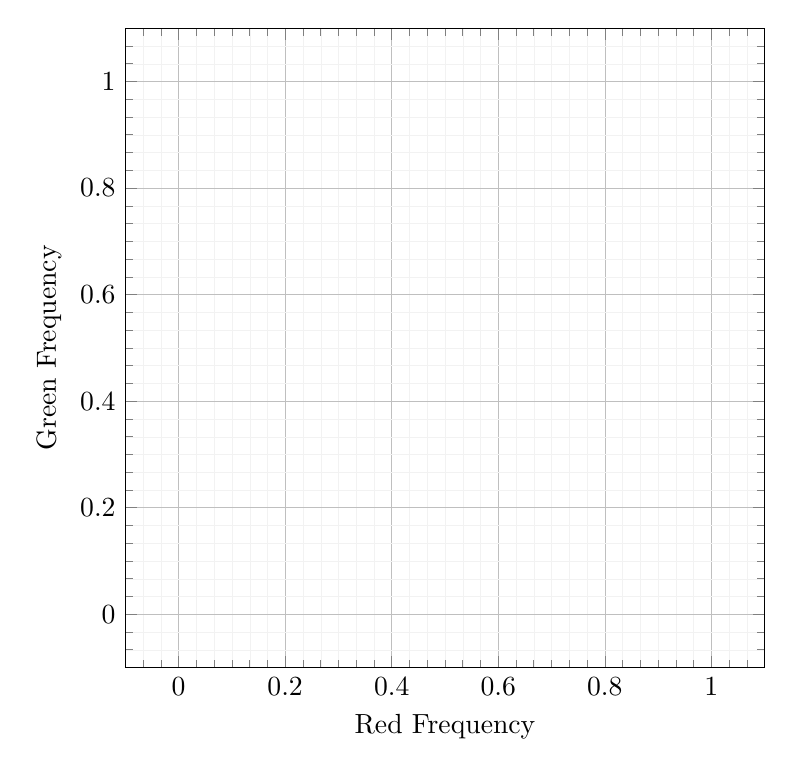
\begin{tikzpicture}
        \begin{axis}[
            xlabel={Red Frequency},
            ylabel={Green Frequency},
            zlabel={Blue Frequency},
            xlabel style={sloped like x axis}, % Make x label follow the x axis
            ylabel style={sloped like y axis}, % Make y label follow the y axis
            zlabel style={sloped}, % Make z label follow the z axis or make it vertical
            legend pos=north west,
            grid=both,
            grid style={line width=.1pt, draw=gray!10},
            major grid style={line width=.2pt,draw=gray!50},
            minor tick num=5,
            width=0.8\textwidth,
            height=0.8\textwidth,
            view={-80}{45}, % Adjust the view angle for better visualization
        ]
        \IfFileExists{code/output_data/color_sensor_calibration/rightColor.csv}{

            % SEEN point
            \addplot3[only marks, ball color=\seencolor, mark=ball, mark size = \ballsize*1.3, draw opacity = 0] coordinates {(\seenx, \seeny, \seenz)};
            \addlegendentry{Frequencies Read by Sensor}

            % CALIBRATION point
            \addlegendentry{Closest Calibration Point \& Used Color}
            \addplot3[only marks, ball color=blue, mark=ball, mark size = \ballsize*1.3, draw opacity = 1, draw= \seencolor, line width = 0.5mm] coordinates {(\calix, \caliy, \caliz)};

            % Line between the two
            \addplot3[ no marks,thick, line width=0.5mm, color=\seencolor, opacity = 1, -latex] coordinates {(\seenx, \seeny, \seenz) (\calix, \caliy, \caliz)};

            % Determine opacity based on sensor

            \addplot3[
                only marks,
                scatter,
                scatter/classes={
                    RED={mark=ball,ball color= red, draw opacity=0, mark size = 0},
                    BLUE={mark=ball,ball color= blue, draw opacity=0, mark size = \ballsize},
                    GREEN={mark=ball,ball color= green, draw opacity=0, mark size = 0},
                    WHITE={mark=ball,ball color= white, draw opacity=0, mark size = 0},
                    BLACK={mark=ball,ball color= black, draw opacity=0, mark size = \ballsize},
                    YELLOW={mark=ball,ball color= yellow, draw opacity=0, mark size = 0}
                },
                scatter src=explicit symbolic,
            ] table[
                x=Red_Freq,
                y=Green_Freq,
                z=Blue_Freq,
                meta = Color,
                col sep=comma,
            ] {code/output_data/color_sensor_calibration/rightColor.csv};

            % Wall histogram on the left
            \addplot3[
                only marks,
                scatter,
                scatter/classes={
                    RED={mark=*,fill=gray, fill opacity=0, draw opacity=0},
                    BLUE={mark=*,fill=gray, fill opacity=\grayopacity, draw opacity=0},
                    GREEN={mark=*,fill=gray, fill opacity=0, draw opacity=0},
                    WHITE={mark=*,fill=gray, fill opacity=0, draw opacity=0},
                    BLACK={mark=*,fill=gray, fill opacity=\grayopacity, draw opacity=0},
                    YELLOW={mark=*,fill=gray, fill opacity=0, draw opacity=0}
                },
                scatter src=explicit symbolic,
            ] table[
                x = Red_Freq,  % This sets the x-coordinate to 0
                y expr = 800,  % This sets the y-coordinate to 0
                z= Blue_Freq,
                meta = Color,
                col sep=comma,
            ] {code/output_data/color_sensor_calibration/rightColor.csv};

            % Wall histogram on the right
            \addplot3[
                only marks,
                scatter,
                scatter/classes={
                    RED={mark=*,fill=gray, fill opacity=0, draw opacity=0},
                    BLUE={mark=*,fill=gray, fill opacity=\grayopacity, draw opacity=0},
                    GREEN={mark=*,fill=gray, fill opacity=0, draw opacity=0},
                    WHITE={mark=*,fill=gray, fill opacity=0, draw opacity=0},
                    BLACK={mark=*,fill=gray, fill opacity=\grayopacity, draw opacity=0},
                    YELLOW={mark=*,fill=gray, fill opacity=0, draw opacity=0}
                },
                scatter src=explicit symbolic,
            ] table[
                x expr = 750,  % This sets the x-coordinate to 0
                y = Green_Freq,  % This sets the y-coordinate to the back wall
                z= Blue_Freq,
                meta = Color,
                col sep=comma,
            ] {code/output_data/color_sensor_calibration/rightColor.csv};

            % Floor histogram
            \addplot3[
                only marks,
                scatter,
                scatter/classes={
                    RED={mark=*,fill=gray, fill opacity=0, draw opacity=0},
                    BLUE={mark=*,fill=gray, fill opacity=\grayopacity, draw opacity=0},
                    GREEN={mark=*,fill=gray, fill opacity=0, draw opacity=0},
                    WHITE={mark=*,fill=gray, fill opacity=0, draw opacity=0},
                    BLACK={mark=*,fill=gray, fill opacity=\grayopacity, draw opacity=0},
                    YELLOW={mark=*,fill=gray, fill opacity=0, draw opacity=0}
                },
                scatter src=explicit symbolic,
            ] table[
                x = Red_Freq,
                y = Green_Freq,
                z expr = 0,
                meta = Color,
                col sep=comma,
            ] {code/output_data/color_sensor_calibration/rightColor.csv};

            
        }{}
        \end{axis}
    \end{tikzpicture}
    \caption{Visual representation of color matching algorithm.\protect\footnotemark}
    \label{fig:color-calibration-distance-example}
\end{figure}
\footnotetext{The orange dot is the seen color by the sensor, and the nearest calibration point is blue, thus the color seen is set to blue.}

\end{document}

%\documentclass{article}
\usepackage{StyleSheet}
\begin{document}

\section{Code}

\subsection{Sensors}

\subsubsection{Button.h}
\lstinputlisting[caption={Button.h}, label=lst:button-h]{../code/main/sensors/Button.h}

\subsubsection{ColorSensor.h}
\lstinputlisting[caption={ColorSensor.h}, label=lst:colorsensor-h]{../code/main/sensors/ColorSensor.h}

\subsubsection{IRSensorArray.h}
\lstinputlisting[caption={IRSensorArray.h}, label=lst:irsensorarray-h]{../code/main/sensors/IRSensorArray.h}

\subsubsection{Motor.h}
\lstinputlisting[caption={Motor.h}, label=lst:motor-h]{../code/main/sensors/Motor.h}

\subsubsection{MWServo.h}
\lstinputlisting[caption={MWServo.h}, label=lst:mwservo-h]{../code/main/sensors/MWServo.h}

\subsubsection{UltraSonic.h}
\lstinputlisting[caption={UltraSonic.h}, label=lst:ultrasonic-h]{../code/main/sensors/UltraSonic.h}

\subsection{Controls}
\subsubsection{PIDController.h}
\lstinputlisting[caption={PIDController.h}, label=lst:pidcontroller-h]{../code/main/controls/PIDController.h}

\subsubsection{Utils.h}
\lstinputlisting[caption={Utils.h}, label=lst:utils-h]{../code/main/controls/Utils.h}

\subsection{BoxControl.h}
\lstinputlisting[caption={BoxControl.h}, label=lst:boxcontrol-h]{../code/main/BoxControl.h}

\subsection{Initialization.h}
\lstinputlisting[caption={Initialization.h}, label=lst:initialization-h]{../code/main/Initialization.h}

\subsection{LineFollowing.h}
\lstinputlisting[caption={LineFollowing.h}, label=lst:linefollowing-h]{../code/main/LineFollowing.h}

\subsection{Motion.h}
\lstinputlisting[caption={Motion.h}, label=lst:motion-h]{../code/main/Motion.h}

\subsection{ObstacleAvoidance.h}
\lstinputlisting[caption={ObstacleAvoidance.h}, label=lst:obstacleavoidance-h]{../code/main/ObstacleAvoidance.h}

\subsection{PickupPlace.h}
\lstinputlisting[caption={PickupPlace.h}, label=lst:pickupplace-h]{../code/main/PickupPlace.h}

\subsection{main.ino}
\lstinputlisting[caption={main.ino}, label=lst:main-h]{../code/main/main.ino}


\end{document}


\end{document}